\chapter{PHƯƠNG PHÁP ĐỀ XUẤT}
%https://ir.vnulib.edu.vn/bitstream/VNUHCM/32505/2/LeMinhHung.html
% Nhớ thêm trích dẫn tham khảo từ luận văn này (tham khảo về cách trình bày)
\label{Chapter3}
%
Trong chương này, luận văn trình bày chi tiết quá trình phân tích và đề xuất phương pháp phát hiện hình ảnh tạo sinh dựa trên đặc trưng tần số cao. Trước tiên, một số thử nghiệm sơ bộ được tiến hành nhằm khảo sát ảnh hưởng của các thành phần tần số đến hiệu quả phân loại giữa ảnh thật và ảnh tạo sinh. Dựa trên kết quả thu được, chương tiếp tục giới thiệu một kỹ thuật tiền xử lý hiệu quả với chi phí tính toán thấp – bộ lọc thông cao rời rạc \textbf{ADOF} – như một thay thế cho biến đổi Fourier truyền thống.

Tiếp theo, một mô hình phân loại được xây dựng trên nền kiến trúc ResNet~\cite{He2015DeepRL}, kết hợp với khối tiền xử lý tần số để tăng cường khả năng nhận biết các đặc trưng vi mô của ảnh giả. Nhằm đáp ứng yêu cầu triển khai thực tế trên các hệ thống hạn chế tài nguyên, chương này cũng đề xuất một phiên bản rút gọn của mô hình, bằng cách sử dụng kỹ thuật \gls{fbkd}. Phần cuối cùng mô tả chi tiết quy trình huấn luyện và triển khai mô hình trong cả hai giai đoạn: đào tạo và suy luận.
%
\section{Thử nghiệm sơ bộ và tìm hướng tiếp cận}
%
\subsection{Thử nghiệm 1}
%
\begin{figure}[ht!]
	\centering
	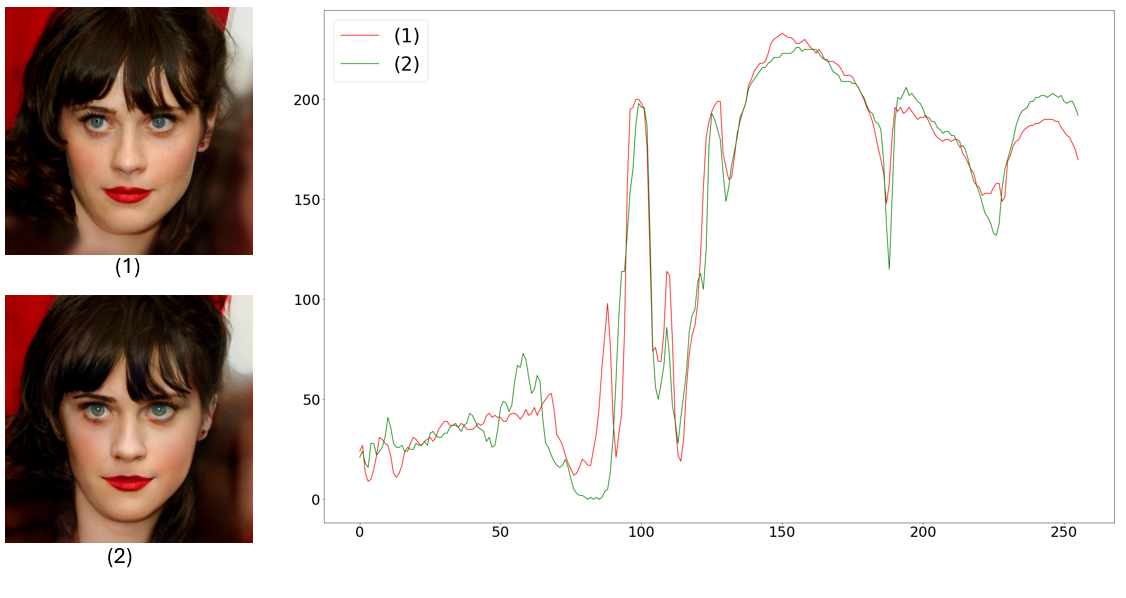
\includegraphics[width=1.0\linewidth]{Images/restyle-encoder-1.png}
	\begin{minipage}{1.0\linewidth}
		\caption{Biểu đồ (\textit{phải}) thể hiện mức xám dòng thứ 100 của ảnh thật (1) và ảnh tạo sinh (2).}
		\label{fig:restyle-encoder-1}
	\end{minipage}
\end{figure}
%
Trong Hình~\ref{fig:restyle-encoder-1}, ta sử dụng ảnh thật (1) lấy từ tập dữ liệu FFHQ và tạo ảnh giả tương ứng (2) bằng phương pháp ReStyle~\cite{alaluf2021restyle}. 
%
Việc sử dụng cặp ảnh thật–giả có cùng đặc điểm khuôn mặt giúp ta khảo sát trực quan độ khó của nhiệm vụ phân biệt hình ảnh tạo sinh. Kết quả cho thấy hai ảnh có mức độ tương đồng cao về hình dáng và chi tiết, gây khó khăn cho việc phân biệt bằng mắt thường.
%
Điều này có thể lý giải bởi thực tế rằng thị giác con người chủ yếu nhận biết thông tin ở các vùng ảnh có kích thước lớn và có độ tương phản cao, trong khi các khác biệt đặc trưng để phân biệt ảnh thật và ảnh tạo sinh rất có thể tồn tại ở mức độ điểm ảnh.
%
%

Các nghiên cứu trước đây \cite{Jeong2021BiHPFBH}, \cite{Frank2020LeveragingFA}, \cite{Jeong2022FrePGANRD} cũng chỉ ra rằng các đặc trưng nhân tạo có xu hướng tập trung ở vùng tần số cao và đã tận dụng điều này để phát triển bộ phân loại dựa trên đặc trưng tần số. Phần~\ref{ssec:thu_nghiem_2}, ta tiến hành thử nghiệm nhằm đánh giá sự ảnh hưởng của đặc trưng tần số đến hiệu xuất bộ phân loại ảnh thật, giả.

\subsection{Thử nghiệm 2}
\label{ssec:thu_nghiem_2}
Bước tiếp theo của quá trình phân tích, ta thực hiện huấn luyện hai bộ phân loại dựa trên kiến trúc ResNet~\cite{He2015DeepRL} và sử dụng cùng bộ dữ liệu \cite{Krizhevsky2012ImageNetCW}.

\textbf{Bộ phân loại số 1:} (Original RGB ) ảnh đầu vào là ảnh màu RGB gốc, giữ nguyên toàn bộ thông tin tần số.  

\textbf{Bộ phân loại số 2:} (Highpass 50\%) Mô hình này sử dụng cùng kiến trúc với Bộ phân loại số 1, tuy nhiên ảnh đầu vào đã được xử lý bằng bộ lọc thông cao, trong đó 50\% thành phần tần số thấp đã bị loại bỏ thông qua biến đổi Fourier. Kết quả huấn luyện được trình bày trong Hình~\ref{fig:Experiment_Highpass50_percent}

%
\begin{figure}[h!]
	\centering
	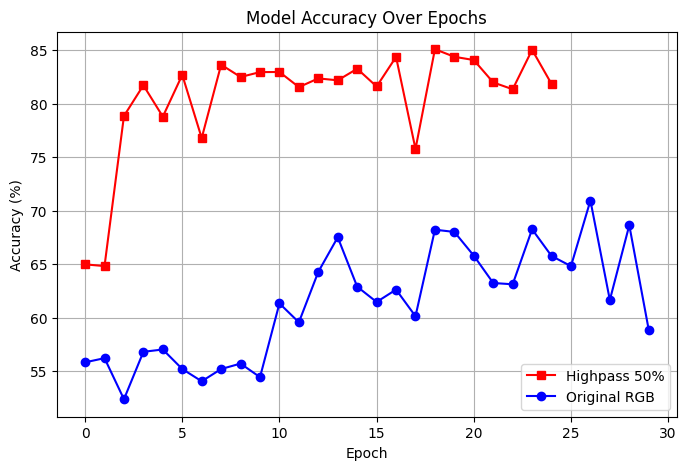
\includegraphics[width=1.0\linewidth]{Images/Experiment_Highpass50_percent.png}
	\begin{minipage}{1.0\linewidth}
		\caption{Độ chính xác của hai bộ phân loại trên tập kiểm tra trong quá trình huấn luyện.}
		\label{fig:Experiment_Highpass50_percent}
	\end{minipage}
\end{figure}

%
Thử nghiệm đã cho thấy các thành phần tần số cao đóng vai trò quan trọng trong quá trình phân loại ảnh thật – giả. Cụ thể, mô hình được huấn luyện trên ảnh đã qua bộ lọc thông cao (Highpass 50\%) đạt độ chính xác cao hơn so với mô hình sử dụng ảnh RGB gốc. Điều này gợi ý rằng thông tin tần số cao chứa các đặc trưng quan trọng giúp phân biệt ảnh giả mạo, trong khi các thành phần tần số thấp có thể chứa nhiều thông tin nền không hữu ích cho quá trình nhận diện.  

\subsection*{Mở rộng thử nghiệm với các mức lọc tần số cao khác nhau}

Nhằm đánh giá thêm tác động của các thành phần tần số cao trong việc phân loại ảnh thật và giả, chúng tôi tiếp tục mở rộng thử nghiệm với các mức lọc thông cao khác nhau: 60\%, 70\%, 80\%, và 90\%. Bằng cách này, ta có thể đánh giá ảnh hưởng của các tín hiệu tần số cao đến hiệu xuất của bộ phân loại.

Những quan sát từ thử nghiệm cho thấy rằng việc tăng cường khai thác thông tin ở dải tần số cao có thể mang lại lợi ích đáng kể cho nhiệm vụ phát hiện ảnh tạo sinh. Do đó, \textbf{hướng tiếp cận nghiên cứu trong phần tiếp theo sẽ tập trung vào khai thác đặc trưng tần số cao để cải thiện độ chính xác phân loại.}

\subsection{Các hạn chế khi dùng biến đổi Fourier}

Trong quá trình thử nghiệm, ta đã sử dụng phép biến đổi \gls{fft}~\cite{Arunachalam2013TheFF} để phân tích tín hiệu trong miền tần số và thực hiện việc loại bỏ các thành phần tần số thấp nhằm tập trung khai thác đặc trưng tần số cao. Việc này giúp tăng hiệu quả phân loại ảnh thật và giả mạo. Tuy nhiên, mặc dù \gls{fft} có ưu điểm về tốc độ tính toán nhanh hơn nhiều so với biến đổi \gls{dft}, quá trình áp dụng \gls{fft} và cắt lọc tần số cũng tồn tại những hạn chế nhất định.

\begin{itemize}
	\item Tuy độ phức tạp tính toán chỉ là $O(N\log{N})$ nhưng ta phải thêm bước \gls{ifft} về không gian ảnh ban đầu sau khi áp dụng mặt nạ lọc tần số.
	\item Khó khăn trong việc tối ưu hoá tốc độ bằng tính toán song song tận dụng sức mạnh của \gls{gpu}.
	\item Tốn nhiều tài nguyên bộ nhớ do các biến đổi ở dạng số phức nên yêu cầu thêm bộ nhớ.
	\item Hiệu ứng biên trong biến đổi \gls{fft} làm xuất hiện các tín hiệu nhiễu không mong muốn.
\end{itemize}

\section{Phép sai phân như một bộ lọc thông cao trong miền tần số}

Để khắc phục các hạn chế của \gls{fft} trong việc lọc tần số cao, một hướng tiếp cận thay thế là xây dựng bộ lọc thông cao trực tiếp trong miền không gian ảnh, cho phép loại bỏ thành phần tần số thấp mà không cần thực hiện biến đổi \gls{fft} và biến đổi \gls{fft} ngược.
%
Cách làm này không chỉ giúp giảm độ phức tạp tính toán mà còn phù hợp hơn cho các hệ thống yêu cầu xử lý nhanh, có tài nguyên hạn chế hoặc dễ dàng tính toán song song nếu hệ thống hổ trợ \gls{gpu}.

Trong phần này, tôi sẽ trình bày cơ sở lý thuyết của phương pháp xây dựng bộ lọc thông cao dựa trên việc biến đổi từ một bộ lọc thông thấp đơn giản – cụ thể là bộ lọc trung bình. 
%
Thông qua phân tích đáp ứng tần số, ta sẽ chứng minh rằng thao tác lấy sai phân (hiệu) giữa các điểm ảnh kề nhau có thể được xem như một phép lọc thông cao hiệu quả, với độ phức tạp rất thấp.

\subsection{Bộ Lọc Trung Bình}

Bộ lọc trung bình rời rạc \( h_{\mathrm{LP}}[n] \) có thể được định nghĩa theo công thức:

\[
h[n] =
\begin{cases}
	\frac{1}{M}, & 0 \leq n < M \\
	0, & \text{ngược lại}
\end{cases}
\]

Trong đó, \( M \) là kích thước của cửa sổ trượt. Tín hiệu đầu ra của bộ lọc trung bình được tính bằng:

\[
y_{\mathrm{LP}}[n] = \frac{1}{M} \sum_{k=0}^{M-1} x[n-k]
\]

Để tìm đáp ứng tần số, ta tiến hành biến đổi Fourier rời rạc của bộ lọc:

\[
H_{\mathrm{LP}}(\omega) = \sum_{n=0}^{M-1} \frac{1}{M} e^{-j \omega n} = \frac{1}{M} \cdot \frac{1 - e^{-j M \omega}}{1 - e^{-j \omega}}
\]

Biểu thức này có thể được rút gọn thành:

\[
H_{\mathrm{LP}}(\omega) = \frac{1}{M} e^{-j \omega \frac{M-1}{2}} \cdot \frac{\sin\left(\frac{M \omega}{2}\right)}{\sin\left(\frac{\omega}{2}\right)}
\]

Với biên độ đáp ứng tần số là:

\[
|H_{\mathrm{LP}}(\omega)| = \left| \frac{1}{M} \cdot \frac{\sin\left( \frac{M \omega}{2} \right)}{\sin\left( \frac{\omega}{2} \right)} \right|
\]

\subsection*{Phân Tích Đặc Tính Đáp Ứng Biên Độ}

- Khi \( \omega \to 0 \), theo định lý L'Hopital, ta có:

\[
\lim_{\omega \to 0} |H_{\mathrm{LP}}(\omega)| = 1
\]

- Khi \( \omega \to \pi \), kết quả phụ thuộc vào giá trị của \( M \):

- Với \( M \) chẵn:

\[
\sin\left(\frac{M\pi}{2}\right) = 0 \Rightarrow |H_{\mathrm{LP}}(\pi)| = 0
\]

- Với \( M \) lẻ:

\[
\sin\left(\frac{M\pi}{2}\right) = \pm 1 \Rightarrow |H_{\mathrm{LP}}(\pi)| = \frac{1}{M}
\]

Nhận xét: Để triệt tiêu hoàn toàn tần số cao, ta nên chọn \( M \) chẵn.

\subsection*{Thiết Kế Bộ Lọc Thông Cao}

Bộ lọc thông cao có thể được xây dựng từ bộ lọc thông thấp thông qua một quan hệ tuyến tính. Cụ thể, tín hiệu đầu ra của bộ lọc thông cao là:

\[
y_{\mathrm{HP}}[n] = x[n] - y_{\mathrm{LP}}[n]
\]

Với \( h_{\mathrm{HP}}[n] \) là đáp ứng xung của bộ lọc thông cao, ta có:

\[
h_{\mathrm{HP}}[n] = \delta[n] - h_{\mathrm{LP}}[n]
\]

Đáp ứng tần số của bộ lọc thông cao được cho bởi:

\[
H_{\mathrm{HP}}(\omega) = 1 - H_{\mathrm{LP}}(\omega)
\]

Thay thế biểu thức của \( H_{\mathrm{LP}}(\omega) \), ta có:

\[
H_{\mathrm{HP}}(\omega) = 1 - \frac{1}{M} e^{-j \omega \frac{M-1}{2}} \cdot \frac{\sin\left(\frac{M \omega}{2}\right)}{\sin\left(\frac{\omega}{2}\right)}
\]

Biên độ đáp ứng tần số của bộ lọc thông cao là:

\[
|H_{\mathrm{HP}}(\omega)| = \left| 1 - \frac{1}{M} \cdot \frac{\sin\left( \frac{M \omega}{2} \right)}{\sin\left( \frac{\omega}{2} \right)} \right|
\]

\subsection*{Phân Tích Đặc Tính Đáp Ứng Biên Độ}

\begin{itemize}
	\item Khi \( \omega \to 0 \):
	\[
	|H_{\mathrm{HP}}(0)| = |1 - H(0)| = 0
	\]
	
	\item Khi \( \omega \to \pi \), kết quả cũng phụ thuộc vào giá trị của \( M \):
	
	Với \( M \) chẵn:
	
	\[
	|H_{\mathrm{HP}}(\pi)| = 1 - 0 = 1, \quad \text{toàn bộ tần số cao nhất được bảo toàn}
	\]
	
	Với \( M \) lẻ:
	
	\[
	|H_{\mathrm{HP}}(\pi)| = 1 - \frac{1}{M} < 1, \quad \text{một phần tần số cao nhất bị suy hao}
	\]
\end{itemize}



Nhận xét: Để giữ lại tần số cao nhiều nhất, ta nên chọn \( M \) chẵn.

\subsection*{Cửa Sổ Bộ Lọc Thông Cao}
\label{sec:cua_so_loc_thong_cao}

Từ biểu thức đáp Ứng Xung của Bộ Lọc Thông Cao:

\[
h_{\mathrm{HP}}[n] = \delta[n] - h_{\mathrm{LP}}[n]
\]

Với \( n = 0 \):

\[
h_{\mathrm{HP}}[0] = \delta[0] - h_{\mathrm{LP}}[0] = 1 - \frac{1}{M}
\]

Với \( 1 \leq n < M \):

\[
h_{\mathrm{HP}}[n] = \delta[n] - \frac{1}{M} = 0 - \frac{1}{M} = -\frac{1}{M}
\]

Với \( n \geq M \):

\[
h_{\mathrm{HP}}[n] = \delta[n] - 0 = 0
\]

Do đó, đáp ứng xung của bộ lọc thông cao có dạng:

\[
h_{\mathrm{HP}}[n] =
\begin{cases}
	1 - \frac{1}{M}, & n = 0 \\
	-\frac{1}{M}, & 1 \leq n < M \\
	0, & \text{ngược lại}
\end{cases}
\]

Biểu thức tổng quát cho bộ lọc thông cao có thể được diễn đạt dưới dạng vector độ dài \( M \):

\begin{equation}
	\label{eq:h_HP}
	h_{\mathrm{HP}}[n] = \left[ 1 - \frac{1}{M},\ -\frac{1}{M},\ -\frac{1}{M},\ \ldots,\ -\frac{1}{M} \right]
\end{equation}
%

Bộ lọc thông cao có thể được xây dựng từ bộ lọc trung bình thông qua một phép toán đơn giản. Qua thực nghiệm, ta thấy rằng \( M = 2 \) cho kết quả tối ưu cho mô hình.
%
Với \( M = 2 \), biểu thức cho đáp ứng xung của bộ lọc thông cao từ phương trình \eqref{eq:h_HP} trở thành:

\[
h_{\mathrm{HP}}[n] = \left[ \frac{1}{2},\ -\frac{1}{2} \right]
\]

Ta thấy rằng đây chính là {phép sai phân tuyến tính chuẩn hóa}, tương đương với:

\[
y[n] = \frac{1}{2}x[n] - \frac{1}{2}x[n-1] = \frac{1}{2}(x[n] - x[n-1])
\]

Bỏ hệ số tỉ lệ (vì không làm thay đổi đặc tính tần số), ta có thể viết lại thành dạng sai phân đơn giản:

\begin{equation}
	\label{eq:y_n}
	y[n] = x[n] - x[n-1]
\end{equation}

Điều này chứng minh rằng khi \( M = 2 \), bộ lọc thông cao được xây dựng từ bộ lọc trung bình chính là \textbf{phép sai phân bậc nhất} – một bộ lọc thông cao hiệu quả với độ phức tạp tính toán rất thấp, đồng thời loại bỏ mạnh mẽ các thành phần tần số thấp trong tín hiệu hoặc ảnh đầu vào.

%
\section{Xây dựng khối tiền xử lý dựa trên bộ lọc thông cao}
Phương trình~\eqref{eq:y_n} mô tả bộ lọc thông cao dưới dạng tổng quát. Ta mở rộng thành ma trận $H_x, H_y$ như bên dưới để thuận tiện cho việc sử dụng thư viện như \texttt{Pytorch} khi lập trình.
	\[
	H_x = \begin{bmatrix}
		0 & 0 & 0 \\
		0 & 1 &  \text{-}1 \\
		0 & 0 & 0
	\end{bmatrix} \qquad \qquad
	H_y = \begin{bmatrix}
		0 & 0 & 0 \\
		0 & 1 &  0 \\
		0 & \text{-}1 & 0
	\end{bmatrix}
	\]
	
Dựa trên phân tích tại mục \ref{sec:cua_so_loc_thong_cao}, ta chọn độ dài cửa sổ lọc $M=2$ vì giá trị $M$ chẵn giữ lại vùng tần số cao tốt hơn so với giá trị lẻ. Đồng thời, lựa chọn $M$ nhỏ giúp giảm chi phí tính toán.

\section{Mô hình đề xuất}

Trong đề tài này, mục tiêu hướng đến là xây dựng một phương pháp có cấu trúc đơn giản, tối ưu về tốc độ xử lý, và phù hợp với các hệ thống có tài nguyên hạn chế trong nhiệm vụ phát hiện hình ảnh tạo sinh. Để đạt được mục tiêu này, kiến trúc ResNet~\cite{He2015DeepRL} được lựa chọn làm nền tảng cho mô hình phân loại.

ResNet~\cite{He2015DeepRL} là một trong những kiến trúc \gls{cnn} hiệu quả nhất được đề xuất bởi He et al. (2015), nổi bật nhờ cơ chế \gls{skipconnection}, cơ chế này cho phép huấn luyện các mô hình có chiều sâu lớn hơn mà vẫn duy trì hiệu quả hội tụ, đồng thời hạn chế hiện tượng mất mát thông tin trong quá trình lan truyền ngược.

So với các kiến trúc phức tạp hơn như EfficientNet~\cite{zhong2024patchcraftexploringtexturepatch}, Vision Transformer~\cite{dosovitskiy2020image}, ResNet có ưu điểm là dễ triển khai, ít tham số hơn, và có thể tùy chỉnh dễ dàng số lượng tầng để phù hợp với yêu cầu tính toán của hệ thống. Trong phạm vi nghiên cứu này, một phiên bản rút gọn từ ResNet-50~\cite{He2015DeepRL} được sử dụng nhằm đảm bảo cân bằng giữa độ chính xác và chi phí tính toán.

Bên cạnh đó, ResNet~\cite{He2015DeepRL} cũng cho thấy khả năng trích xuất đặc trưng tốt ở các tác vụ phân biệt hình ảnh có sai khác nhỏ, chẳng hạn như sự khác biệt vi mô giữa ảnh thật và ảnh tạo sinh – điều này đặc biệt quan trọng trong bối cảnh \gls{deepfake} ngày càng tinh vi.

\subsection{Kiến trúc mô hình rút gọn từ ResNet-50}
\label{sec:kien_truc_mo_hinh_rut_gon_tu_resnet_50}
Mô hình đề xuất được mô tả trong Hình~\ref{fig:figure_model_architecture}), trong đó chỉ sử dụng hai khối residual đầu tiên của kiến trúc ResNet-50 (tương ứng với \texttt{Layer1} và \texttt{Layer2}) để thực hiện trích xuất đặc trưng, kết hợp với một bộ phân loại nhị phân đơn giản ở đầu ra. Việc tinh giản này giúp giảm số lượng tham số từ khoảng 23 triệu (của ResNet-50 đầy đủ) xuống còn khoảng 1.4 triệu tham số. Mô hình bao gồm các thành phần chính như sau:
%
\begin{figure}[h!]
	\centering
	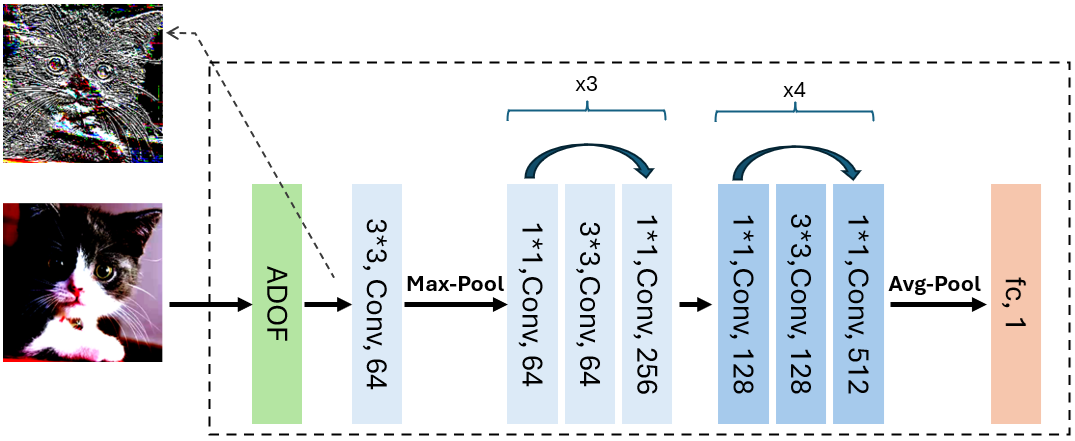
\includegraphics[width=1.0\linewidth]{Images/figure_model_architecture.png}
	\begin{minipage}{1.0\linewidth}
		\vspace{5mm}
		\caption{Kiến trúc mạng Resnet-50 rút gọn}
		\label{fig:figure_model_architecture}
	\end{minipage}
\end{figure}
%
%

\begin{itemize}
	\item \textbf{Khối tiền xử lý ADOF}
	
	Phương trình~\eqref{eq:h_HP} mô tả bộ lọc thông cao dưới dạng tổng quát. Ta mở rộng thành ma trận $H_x, H_y$ như bên dưới để thuận tiện cho việc sử dụng thư viện như \texttt{Pytorch} khi lập trình.
	\[
		H_x = \begin{bmatrix}
			0 & 0 & 0 \\
			0 & \tfrac{1}{2} &  \text{-}\tfrac{1}{2} \\
			0 & 0 & 0
		\end{bmatrix} \qquad \qquad
		H_y = \begin{bmatrix}
			0 & 0 & 0 \\
			0 & \tfrac{1}{2} &  0 \\
			0 & \text{-}\tfrac{1}{2} & 0
		\end{bmatrix}
	\]
	
		\begin{itemize}
			\item Hai 2 bộ lọc thông cao áp dụng cho 2 hướng $x, y$ giúp loại bỏ thông tin tần số thấp của hình ảnh.
			\item Đầu ra tương ứng của 2 bộ lọc thông cao được kết hợp với nhau để tạo ra một bản đồ đặt trưng. \textcolor{red}{Chi tiết được trình bài tại..}
		\end{itemize}

%
	\item \textbf{Tầng đầu vào}:
	%
		\begin{itemize}
			\item Một lớp \gls{convolution} với \gls{kernel} kích thước \(3 \times 3\), \gls{stride} = 2, \gls{padding} = 1, không dùng \texttt{bias}.
			\item Tiếp theo là lớp \gls{batchnorm} và hàm kích hoạt \gls{relu}.
			\item Sau cùng là lớp \gls{maxpooling} với \gls{kernel} \(3 \times 3\), \gls{stride} = 2, \gls{padding} = 1.
		\end{itemize}
		%
		\item \textbf{Tầng \texttt{layer1}}:
		\begin{itemize}
			\item Gồm 3 khối \gls{bottleneck}, được kết nối bằng \gls{skipconnection}, nhằm học các đặc trưng cơ bản như biên cạnh, vùng chuyển tiếp và kết cấu bề mặt ảnh.
		\end{itemize}
		
		\item \textbf{Tầng \texttt{layer2}}:
		\begin{itemize}
			\item Gồm 4 khối \gls{bottleneck}, tiếp tục trích xuất đặc trưng ở mức trừu tượng cao hơn, giúp mô hình nhận diện các khác biệt tinh vi giữa ảnh thật và ảnh tạo sinh.
		\end{itemize}
		
		\item \textbf{Bộ phân loại đầu ra}:
		\begin{itemize}
			\item Một lớp \gls{gap} để chuyển đổi bản đồ đặc trưng thành vector đặc trưng cố định chiều.
			\item Một lớp \gls{fc} với một nút đầu ra duy nhất, sử dụng hàm kích hoạt \gls{sigmoid} để phân loại ảnh đầu vào là thật hay tạo sinh.
		\end{itemize}
\end{itemize}

\subsection{Hàm mất mát}
\label{ss:ham_mat_mat_bce}
Để huấn luyện mô hình phân loại ảnh thật và ảnh tạo sinh, luận văn sử dụng hàm mất mát nhị phân \gls{bce}, được định nghĩa như sau:

\begin{equation}
	\mathcal{L}_{\mathrm{BCE}} = -\frac{1}{N} \sum_{i=1}^{N} \left[ y_i \log(\hat{y}_i) + (1 - y_i)\log(1 - \hat{y}_i) \right]
\end{equation}

Trong đó, \( y_i \in \{0, 1\} \) là nhãn thực tế của ảnh đầu vào, và \( \hat{y}_i \in (0, 1) \) là xác suất do mô hình dự đoán.

\subsection{Quy trình huấn luyện và sử dụng}
%
\label{ssec:quy_trinh_huan_luyen}
%
Quá trình huấn luyện được mô tả trong Hình~\ref{fig:offline-training-process}, ảnh đầu vào sẽ được chuẩn hóa và tiền xử lý nhằm đồng nhất kích thước, tăng tính đa dạng qua các kỹ thuật tăng cường dữ liệu xoay và lật ảnh. Sau bước này, ảnh được đưa qua khối \textcolor{red}{ADOF} – có chức năng lọc lấy những tín hiệu ở tần số cao trong ảnh, nơi mà các mô hình tạo sinh thường để lại dấu vết.
%
\begin{figure}[h!]
	\centering
	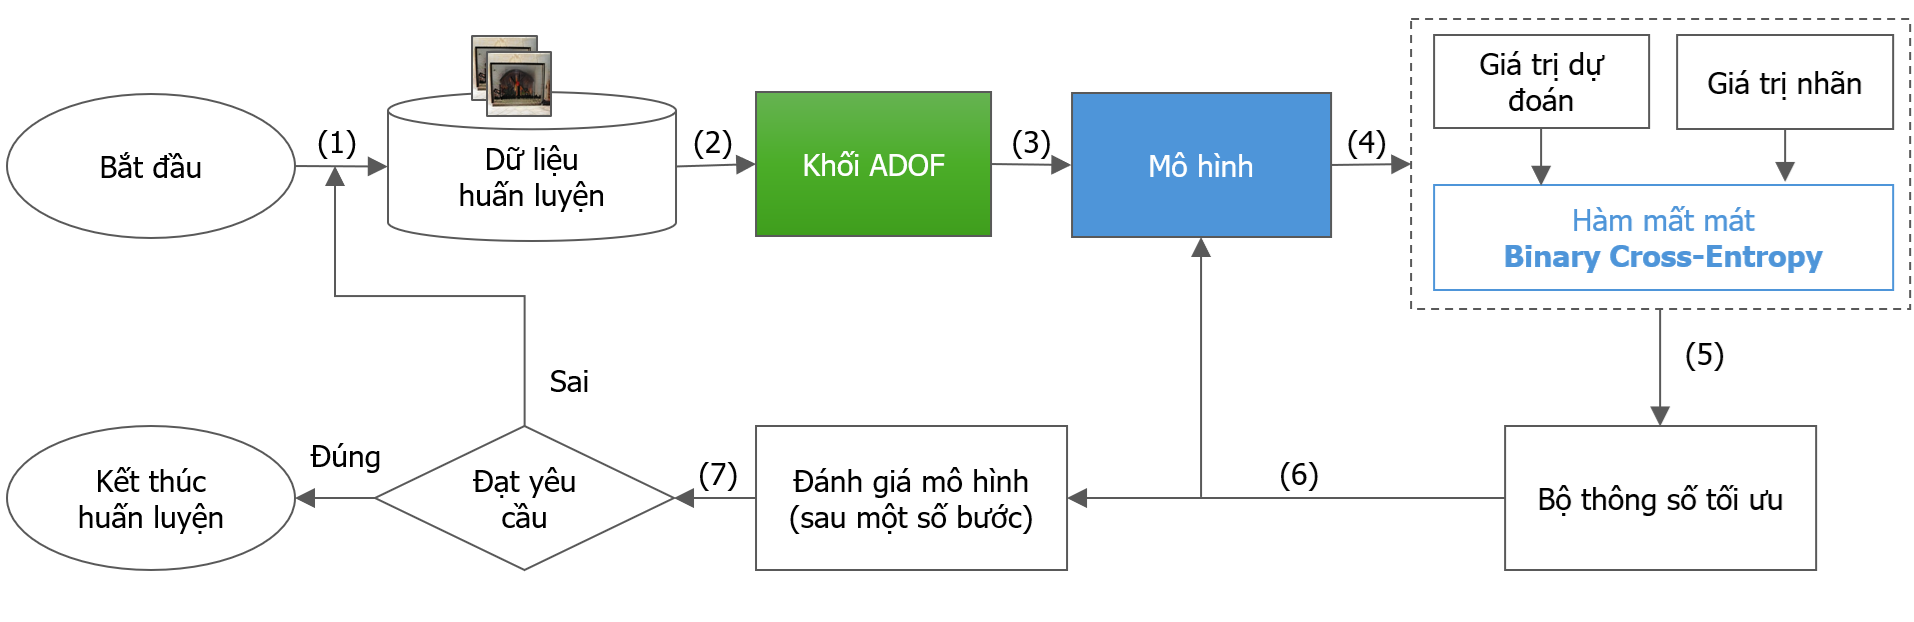
\includegraphics[width=1.0\linewidth]{Images/offline-training-process.png}
	\begin{minipage}{1.0\linewidth}
		\vspace{3mm}
		\caption{Quy trình huấn luyện}
		\label{fig:offline-training-process}
	\end{minipage}
\end{figure}
%
Đầu ra từ khối \textcolor{red}{ADOF} sau đó được đưa vào một kiến trúc ResNet-50~\cite{He2015DeepRL} đã được rút gọn và điều chỉnh nhằm trích xuất đặc trưng và thực hiện phân loại. Kiến trúc này được giảm bớt số lượng tầng so với phiên bản đầy đủ để giảm chi phí tính toán nhưng vẫn giữ lại khả năng biểu diễn cần thiết cho bài toán nhị phân. Đầu ra cuối cùng của mạng là một giá trị xác suất thể hiện mức độ tin tưởng rằng ảnh đầu vào là ảnh tạo sinh. Hàm mất mát được sử dụng trong quá trình huấn luyện là \gls{bce}, kết hợp với thuật toán tối ưu \gls{adam}. Sự lựa chọn này đặc biệt phù hợp với bài toán phân loại nhị phân, giúp mô hình hội tụ nhanh và ổn định. 

Quá trình huấn luyện được tổ chức thành nhiều bước cập nhật trọng số trong mỗi \gls{epoch}. Mỗi bước tương ứng với một \gls{batch} dữ liệu được đưa vào mô hình để tính toán hàm mất mát và cập nhật trọng số thông qua lan truyền ngược. Sau khi hoàn tất một \gls{epoch} – tức là toàn bộ tập huấn luyện đã được xử lý – mô hình sẽ được đánh giá trên tập dữ liệu kiểm thử nhằm theo dõi hiệu năng tổng thể và điều chỉnh chiến lược huấn luyện nếu cần thiết. Quá trình này tiếp tục cho đến khi mô hình đạt đến số \gls{epoch} tối đa đã định hoặc khi các chỉ số đánh giá dừng cải thiện trong một khoảng thời gian xác định trước. Quy trình huấn luyện như trên giúp mô hình học được các đặc trưng phân biệt hiệu quả giữa ảnh thật và ảnh tạo sinh, đồng thời hạn chế hiện tượng \gls{overfitting}.
%
%
\begin{figure}[ht!]
	\centering
	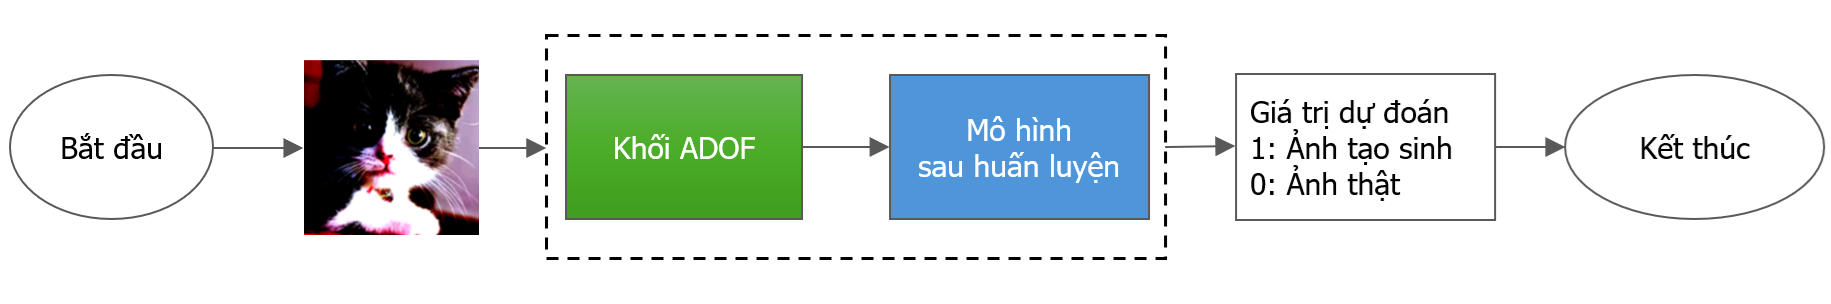
\includegraphics[width=1.0\linewidth]{Images/online-serving.png}
	\begin{minipage}{1.0\linewidth}
		\vspace{3mm}
		\caption{Quy trình sử dụng}
		\label{fig:online-serving}
	\end{minipage}
\end{figure}
%
%

Sau khi quá trình huấn luyện hoàn tất, mô hình đã sẵn sàng cho việc dự đoán trên dữ liệu mới (chi tiết được mô tả trong Hình~\ref{fig:online-serving}). Trong giai đoạn này, ảnh đầu vào sẽ được chuẩn hoá theo đúng các thông số đã sử dụng trong quá trình huấn luyện nhằm đảm bảo tính nhất quán về phân phối dữ liệu. Tiếp theo, ảnh được đưa qua khối \textcolor{red}{ADOF} để trích xuất các tín hiệu tần số cao. Đầu ra từ khối này được chuyển vào mô hình đã huấn luyện để thực hiện suy luận và đưa ra kết quả dự đoán cuối cùng.

\section{Tối giản mô hình với kỹ thuật \gls{fbkd}}

Nhằm tối ưu khả năng triển khai thực tế trên các thiết bị có tài nguyên hạn chế, sau khi hoàn tất huấn luyện mô hình với kiến trúc trình bày ở phần~\ref{sec:kien_truc_mo_hinh_rut_gon_tu_resnet_50}, ta tiếp tục áp dụng kỹ thuật \gls{fbkd} để rút gọn mô hình.

Cụ thể, mô hình đã huấn luyện sẽ đóng vai trò là mô hình \gls{teacher}, từ đó truyền đạt kiến thức cho một mô hình \gls{student} nhỏ gọn hơn. Thay vì chỉ dựa vào đầu ra cuối cùng, mô hình \gls{student} được hướng dẫn học theo các đặc trưng trung gian từ \gls{teacher}, giúp duy trì hiệu suất nhận dạng trong khi giảm đáng kể kích thước và chi phí suy luận của mô hình.

\subsection{Kiến trúc mô hình \gls{student}}
%figure_model_student_architecture.png
%
%
Trong mô hình \gls{student}, ta chỉ giữ lại một khối \gls{bottleneck} tại \texttt{Layer1} (thay vì ba khối) và một khối \gls{bottleneck} tại \texttt{Layer2} (thay vì bốn khối) từ mô hình \gls{teacher} (Hình~\ref{fig:figure_model_architecture}).
%
Việc lựa chọn số lượng layer được giữ lại trong mô hình \gls{student} là kết quả của quá trình thử nghiệm thực tế, với tiêu chí cân bằng giữa độ chính xác và độ phức tạp của mô hình.
%%
\subsection{Hàm mất mát}

Hàm mất mát trong quá trình huấn luyện mô hình \gls{student} là sự kết hợp của hai thành phần:

\begin{enumerate}
	\item \textbf{Hàm mất mát phân loại (Classification Loss)}:
	%
	Là hàm \gls{bce}, được sử dụng trực tiếp để huấn luyện mô hình \gls{student} theo nhãn thật. Chi tiết về \gls{bce} đã được trình bày tại phần~\ref{ss:ham_mat_mat_bce}.
	%
	%
	\item \textbf{Hàm mất mát lan truyền tri thức (\Gls{distillation} Loss)}:
	%
	Thành phần này được sử dụng để truyền đạt tri thức từ mô hình \gls{teacher} sang \gls{student} thông qua việc so sánh các biểu diễn đặc trưng tại một lớp trung gian, cụ thể là đầu ra của \texttt{Layer2}. Để đo lường mức độ sai khác giữa hai biểu diễn này, ta sử dụng hàm mất mát \gls{mse}.
	%
	\begin{equation}
		\mathcal{L}_{\mathrm{distill}} = \frac{1}{N} \sum_{i=1}^{N} \left\| f^{(T)}_i - f^{(S)}_i \right\|^2
	\end{equation}
	
	trong đó, \( f^{(T)}_i \) và \( f^{(S)}_i \) lần lượt là véc-tơ đặc trưng đầu ra tại lớp trung gian của mô hình \gls{teacher} và \gls{student} ứng với mẫu dữ liệu thứ \( i \).
		
\end{enumerate}

Tổng hàm mất mát được tính theo công thức:
\begin{equation}
	\mathcal{L}_{\mathrm{total}} = \lambda \cdot \mathcal{L}_{\mathrm{distill}} + (1 - \lambda) \cdot \mathcal{L}_{\mathrm{BCE}}
\end{equation}
trong đó \( \lambda \in [0, 1] \) là siêu tham số điều chỉnh mức độ ảnh hưởng của mỗi thành phần trong tổng hàm mất mát. Việc lựa chọn giá trị \( \lambda \) phù hợp được xác định thông qua quá trình hiệu chỉnh và thử nghiệm thực tế.
%
%
\subsection{Quy trình huấn luyện và sử dụng}
%offline-training-process-distillation.png
%
Quy trình huấn luyện trải qua các bước tương tự với như phần~\ref{ssec:quy_trinh_huan_luyen}.
%
Điểm khác biệt nằm ở quá trình lan truyền thuận, hàm mất mát và việc cập nhật bộ trọng số cho mô hình.
%
%
\begin{figure}[h!]
	\centering
	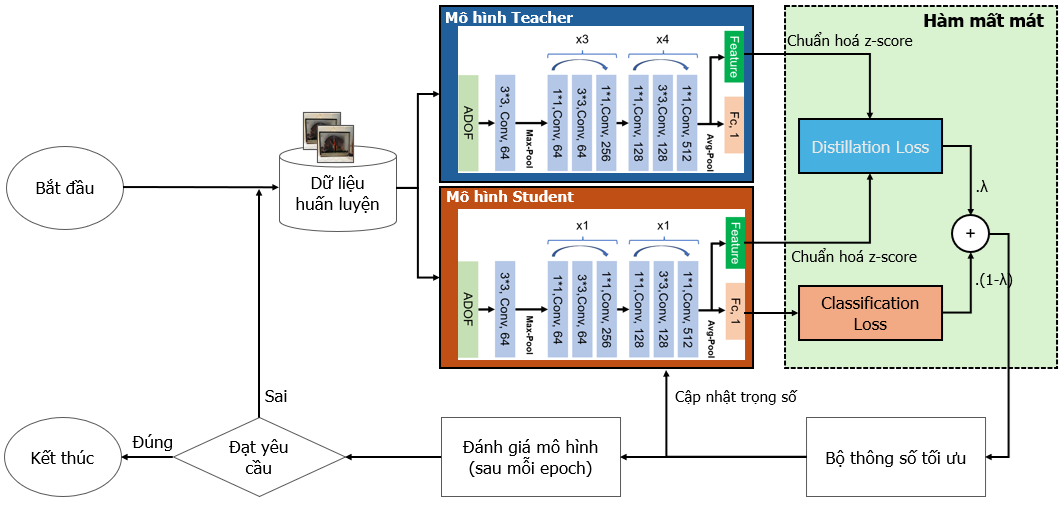
\includegraphics[width=1.0\linewidth]{Images/offline-training-process-distillation.png}
	\begin{minipage}{1.0\linewidth}
		\vspace{5mm}
		\caption{Quy trình huấn luyện mô hình áp dụng kỹ thuật Knowledge-Distillation}
		\label{fig:offline-training-process-distillation}
	\end{minipage}
\end{figure}
%
\begin{itemize}
	\item Lan truyền thuận: Hình ảnh từ đầu vào sẽ được đi qua cả hai mô hình \gls{teacher} và \gls{student}. Sau đó ta trích xuất véc-tơ đặc trưng ở đầu ra của \texttt{Layer2} trong mỗi mô hình và đưa vào hàm mất mát.
	
	\item  Tối ưu hàm mất mát: Là sự kết hợp của 2 hàm mất mát thành phần \gls{distillation} và \gls{classification}.
%	chi tiết được trình bày tại \textcolor{red}{tham chiều tới..}
	
	\item Cập nhật trọng số: Trong suốt quá trình huấn luyện, mô hình \gls{teacher} chỉ sử dụng duy nhất một bộ trọng số đã được huấn luyện trước. Việc cập nhật bộ trọng số chỉ được áp dụng cho mô hình \gls{student}.
\end{itemize}

Sau khi quá trình huấn luyện hoàn tất, mô hình \gls{student} đã sẵn sàng cho việc dự đoán trên dữ liệu mới (chi tiết xem trên Hình~\ref{fig:online-serving}). 







